% !TEX root = ../thesis-example.tex
%
\chapter{Konzept des Evaluations-Rahmenwerks}
\label{sec:konzept}

In diesem Kapitel wird das Konzept vorgestellt, nach dem das Evaluations-Rahmenwerk entwickelt wurde. In Abbildung \ref{fig:konzept-aufbau} wird dargestellt, wie die Leistung eines Parsers evaluiert wird. Der Input-Text ist der rohe Text, den der Parser mit syntaktischer Annotation versehen soll. Das Parser-Modell ist die Grundlage auf der ein Parser arbeitet. Der \textit{Goldstandard} ist der Input-Text mit - als korrekt angesehener - Annotation. Dieser wird mit der Ausgabe des Parsers verglichen. Daraus lassen sich Kennzahlen zur Leistung des Parsers errechnen, die am Ende ausgegeben werden.
Um mehrere Parser miteinander zu vergleichen, werden die Resultate der einzelnen in einer Tabelle zusammengefasst und dargestellt. Alle Elemente werden nachfolgend ausführlich vorgestellt. 
\begin{figure} [h]

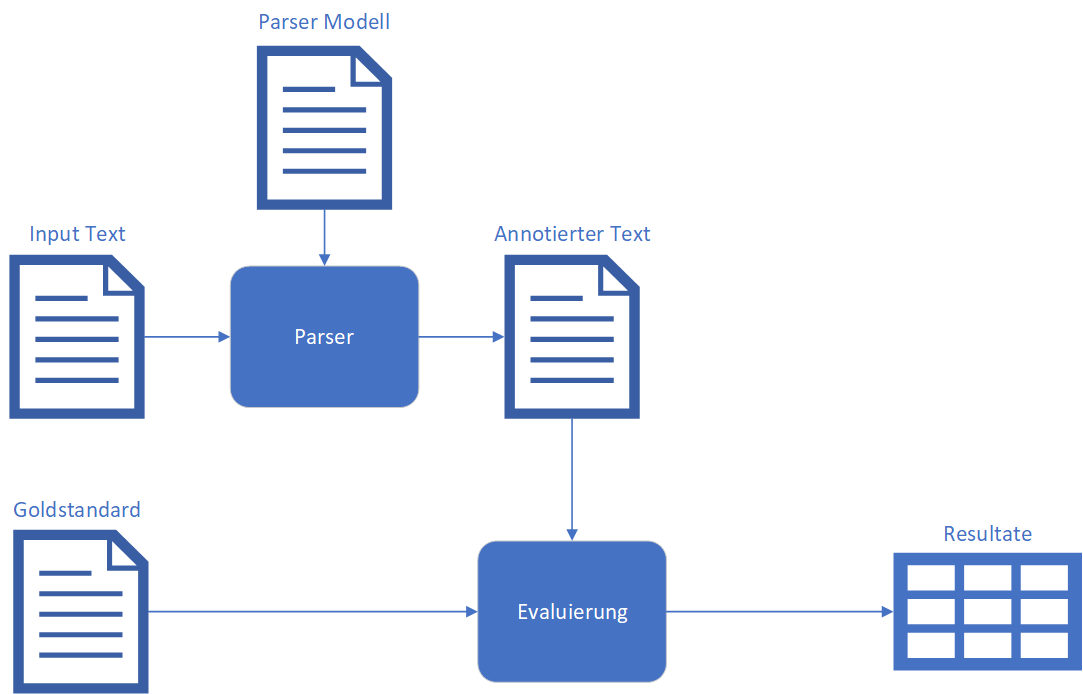
\includegraphics[width=\textwidth]{gfx/konzept-aufbau-png.png} 
\label{fig:konzept-aufbau}	
\caption{Konzeptueller Aufbau}	
\end{figure}
		
\section{Input Text}

Die Eingabe des Parser ist nicht der eigentliche natürlich-sprachliche Text. Ein Element des Satzes, dem ein \textit{POS-Tag} zugewiesen wird, heißt \textit{Token}. In den Eingabesätzen müssen bereits alle \textit{Token} durch Leerzeichen getrennt. Ein solcher Satz wird \textit{sequenziert} genannt. In den meisten Fällen haben die \textit{Token} bereits die benötigten Leerzeichen vor und hinter sich. Ein Beispiel, indem das nicht der Fall ist, ist \textit{he's}. Hier erkennt der Parser nur dass es sich um die Wörter \textit{he} und \textit{is} handelt, wenn ein Leerzeichen vor dem Apostroph eingeschoben wird. Bekommt man aus einem Korpus keine Version des Satzes, bei dem dieser Arbeitsschritt schon erledigt ist, muss man einen \textit{Tokenizer} vorschalten. Das ist ein Programm, welches Eingabesätze sequenziert. Hierfür gibt es unterschiedliche Anbieter, wie zum Beispiel Stanford \cite{stanfordTokenizer} oder OpenNLP \cite{openNlpManual}. %TODO Zitieren https://nlp.stanford.edu/software/tokenizer.html und http://opennlp.sourceforge.net/api/opennlp/tools/tokenize/Tokenizer.html
Allerdings wird in der Implementierung kein \textit{Tokenizer} verwendet. \\
Die Sätze der Eingabe müssen über ein Textdokument übergeben und zeilenweise getrennt sein. Der Parser erstellt für jede Zeile einen Syntaxbaum.

\section{Parser Output}
Als Ausgabe gibt der Parser die annotierten Sätze in der Reihenfolge, in der sie eingegeben wurden, zurück. Es wird hierfür wieder ein Textdokument erstellt. % Bei manchen Parsern besteht die Möglichkeit für einen Satz die \textit{n} besten Bäume ausgeben zulassen. %TODO Entweder top n implementieren oder erklären wieso nicht implementiert und was man damit machen kann
Beispielsweise lautet die annotierten Version des Satzes
\begin{quote}
It goes 150 miles an hour .
\end{quote}
\begin{quote}
( (S (NP (PRP It)) (VP (VBZ goes) (NP (NP (CD 150) (NNS miles)) \\(NP (DT an) (NN hour)))) (. .)) )
\end{quote}
Das äußerste Klammerpaar hat kein führendes Nichtterminal und könnte deshalb weggelassen werden. Es enthält typischerweise das Startsymbol der Parser, also \textit{ROOT}, \textit{TOP} oder ähnliches. Dieses Nichtterminal wird aber für die Evaluierung aus dem Ergebnisbaum herausgenommen, weil es keine syntaktische Information liefert. Da der Satz des \textit{Goldstandards} ebenfalls diese unannotierten Klammern besitzt, werden sie aus beiden Bäumen nicht gelöscht sondern im Evaluationsschritt ignoriert.
\section{Parser Modell}
Das Modell des Parser ist in der Regel eine lexikalisierte oder unlexikalisierte \textit{PCFG}. Die Wahrscheinlichkeitswerte einer \textit{PCFG} sind ausschlaggebend für die Leistung der Parser. Deshalb  erzielt ein Parser, je nachdem welches Modell ihm zu Grunde liegt, sehr unterschiedliche Ergebnisse. Aus diesem Grund ist dieses Modell nicht fest im Parser verankert, sondern wird ihm als Datei übergeben. Somit kann man selbst Modelle anhand einer \textit{Treebank} erstellen lassen um dann beispielsweise auf einem Parser die unterschiedlichen Modelle zu vergleichen. Alle verwendeten Parser bringen ein trainiertes Modell mit.  %TODO für die verwendeten Parser gibt es bereits erstelle Modelle die mit der ... Treebank trainiert wurden. Diese werden eingesetzt.

\section{Goldstandard}
Als \textit{Goldstandard} werden die korrekten Bäume bezeichnet. Diese wurden entweder von Menschenhand erstellt oder durch einen Parser produziert und dann von Menschen nachkorrigiert. Es muss für ein eingegebenes Textdokument, welches vom Parser bearbeitet werden soll auch ein Textdokument geben, das für jeden dieser Sätze die annotierte Version enthält. Die gratis verfügbaren \textit{Treebanks} weisen oft ein unterschiedliches Sortiment an Dateien und Formaten auf.\\
Der in dieser Arbeit verwendete Korpus heißt ``The NAIST-NTT TED Talk Treebank'' \cite{tedtalks} und stammt aus dem Jahr 2014. Er umfasst etwa 23.000 Wörter in 1.200 Sätzen, welche aus 10 Reden gewonnen wurden. Zur Annotierung wurde der Berkeley Parser verwendet und dessen Resultat per Hand verbessert. Als \textit{Tagset} wurde die Vorlage der \textit{Penn Treebank} verwendet. 
%TODO zitat paper ted talk treebank und ein zwei Sätze über diesen verlieren und sagen, dass goldstandard bedeutet zu ca 99 prozent korrekt....
In dieser \textit{Treebank} sind für jeden Satz eine Rohversion, eine sequenzierte und eine annotierte Version enthalten. Rohversion ist der unveränderte, natürlich-sprachliche Satz. Da es sich bei den Texten um Gesprochenes handelt, sind noch weitere Informationen, wie zum Beispiel Zeitmessung eines Satzes und ähnliches vorhanden. Das wird hier nicht weiter verwendet.\\
Bei Verwendung anderer \textit{Goldstandards} können diverse Probleme auftreten. Zwei davon sind hier kurz durchdacht aber nicht implementiert worden.\\
Falls das Problem auftritt, dass nur die korrekten Lösungsbäume zur Eingabe verfügbar sind, so kann man sich zum Beispiel mit dem Python Toolkit NLTK \cite{nltk} %TODO Nltk verlinken
die Blätter jedes Lösungsbaums ausgeben lassen. Hierdurch erhält man, den in seine Token aufgeteilten Satz.\\
Ist der Lösungsbaum nicht einzeilig, sondern erstreckt sich ähnlich zu Abbildung \ref{fig:multiline-annotated-dog-eating}  über mehrere Zeilen, so muss hier auch eine Vorverarbeitung geschehen. Entweder kann anhand der Klammerung erkannt werden wo die Grenzen des Baumes liegen oder es müssen alle Zeilen, die mit einer Art Leerzeichen (Tabulator, u.ä.) beginnen, an die vorherige gehangen werden.

\section{Parser}

Alle Parser erhalten die Eingabe in selber Form, allerdings kann jeder Parser noch eine individuelle Vorverarbeitung benötigen. Dazu mehr in Abschnitt \ref{sec:impl:eigene}.
Im Rahmen dieser Arbeit sind drei Parser verglichen worden. Das sind der \textit{Stanford-Parser} \cite{stanfordparser}, der \textit{Berkeley-Parser} \cite{berkeleyparser1} und der Parser aus dem \textit{OpenNLP Paket} \cite{openNlpManual}. Jeder verwendet zum Annotieren die \textit{Penn Treebank Tags} und liefert die Ausgabe standardmäßig ohne die zusätzlichen relationalen \textit{Tags}. 
%TODO erklären dass keine Dependency parser verwendet werden und was das ist (evtl in kapitel grundlagen), erklären dass alle selbes Tagset verwenden und das keine relational tags verwendet werden
%TODO WICHTIG: Was entscheidet ob der Parser gut ist? nur modell oder noch mehr? warum also nicht nur modelle entwickeln, sondern ganze parser?? liegt auch an algorithmus zum finden baumes vermutlich (cky, earley, ...) besser informieren darüber!

\section{Evaluierung}
\label{sec:konzept:eval}
Für die Evaluierung wird das Ergebnis der Parser zeilenweise mit dem \textit{Goldstandard} verglichen. Zu diesem Zweck werden die Konstituenten der Bäume betrachtet. Eine Konstituente beschreibt einen Knoten im Baum und enthält die Information über das Nichtterminal, den Start- und den Endpunkt. Die Punkte geben den Index des ersten und letzten Wortes dieses Teilbaums an. Mit jedem Wort wird der Zähler inkrementiert. Für den Beispielsatz \textit{They learn much faster.} (Baum in Abbildung \ref{fig:korrekter-baum-eval}) sind die Konstituenten in Tabelle \ref{tab:konstituenten-korrekter-baum-eval} dargestellt. \\
\begin{figure} [h]
\qtreecentertrue\Tree [.S [.NP [.PRP They ] ] [.VP [.VBP learn ] [.S [.ADJP [.RB much ] [.RBR faster ] ] ] ] [.. . ] ]
\caption{Syntaxbaum zu \textit{They learn much faster.}}
\label{fig:korrekter-baum-eval}
\end{figure}
\begin{table} [h]
\centering
\begin{tabular}{ | l | l | l | l |}
	\hline
	Nichtterminal & Text & Start & Ende \\
	\hline
	S & They learn much faster . & 0 & 5 \\
	NP & They & 0 & 1 \\
	PRP & They & 0 & 1 \\
	VP & learn much faster & 1 & 4 \\
	VBD & learn & 1 & 2 \\
	S & much faster & 2 & 4 \\
	ADJP & much faster & 2 & 4 \\
	RB & much & 2 & 3 \\
	RBR & faster & 3 & 4 \\
	. & . & 4 & 5 \\
	\hline
	
\end{tabular}
\caption{Konstituenten zu Abbildung \ref{fig:korrekter-baum-eval}}
\label{tab:konstituenten-korrekter-baum-eval}
\end{table}
Falls es, für eine Konstituente des Parsers, im \textit{Goldstandard} eine mit gleichem Nichtterminal und gleicher Spanne gibt, wird diese als richtig bewertet. Hier muss bei der Ausführung entschieden werden, welche Nichtterminale gewertet werden. Zum einen kann man alle in das Resultat einbeziehen. Zum anderen können die \textit{POS-Tags} herausgelassen und nur die syntaktischen \textit{Tags} aus Tabelle \ref{tab:phrase-tags} bewertet werden. Der Grund ist, dass man so Parser einbringen kann, die als Eingabe einen mit \textit{POS-Tags} versehenen Text bekommen. Diese \textit{Tags} verfälschen dann die Korrektheitsrate der Parser und müssen ignoriert werden. Da in dieser Arbeit ausschließlich Parser genutzt werden, die als Eingabe sequenzierten Text bekommen, betrachten wir hier den Fall in dem alle \textit{Tags} relevant sind. Der Evaluierungsmechanismus ist angelehnt an \cite{parseval}, bzw. \cite{crossbrackets}. %TODO Zitieren Paper Parseval und dessen Quelle und Buch kap 12
Als Bewertungsmetriken werden folgende vier Werte errechnet: \textit{Precision}, \textit{Recall}, \(F_1\) und \textit{Relative Cross Brackets} (kurz: RCB). Siehe Formeln (\ref{eqn:precision}) bis (\ref{eqn:rcb}). \\ 
\begin{equation}
Precision = \frac{\# \;\; korrekte \;\; Konstituenten}{ \# \;\; Konstituenten \;\; im \;\; Parseroutput}
\label{eqn:precision}
\end{equation}

\begin{equation}
Recall = \frac{\# \;\; korrekte \;\; Konstituenten}{ \# \;\; Konstituenten \;\; im \;\; Goldstandard}
\end{equation}

\begin{equation}
F_1 = \frac{2 \times Precision \times Recall}{ Precision + Recall}
\end{equation}

\begin{equation}
RCB = \frac{\# \; Parser \; Konst. \; die \; Goldstandard \; Konst. \; kreuzen}{ \# \;\; Konst. \;\; im \;\; Parseroutput}
\label{eqn:rcb}
\end{equation}

Die \textit{Precision}, im Deutschen \textit{Genauigkeit}, gibt an, wieviele der Konstituenten des Parsers korrekt sind. \textit{Recall}, oder \textit{Trefferquote}, beschreibt zu welchem Teil die Konsituenten des \textit{Goldstandards} mit den Parser-Konstituenten abgedeckt wurden. \(F_\alpha\) ist das gewichtete harmonische Mittel aus beiden. Im Rahmen dieser Arbeit wurde nur \(F_1\) betrachtet, d.h. beide werden gleich gewichtet. Beim \textit{RCB}-Wert handelt es sich um einen Indikator, der ausschließlich für Syntaxbäume eingesetzt wird und vorgestellt wurde in \cite{crossbrackets}. Er gibt an, wieviele der Konstituenten des Parsers sich mit denen des Standards kreuzen. Kreuzen ist in diesem Kontext folgendermaßen definiert: Seien \textit{k1} und \textit{k2} zwei Konstituenten mit unterschiedlichen Start- und Endpunkten. Außerdem gilt o.B.d.A., dass \textit{k1} den niedrigeren Startpunkt hat. Dann kreuzen sie, falls der Endpunkt von \textit{k1} größer als der Startpunkt und kleiner als der Endpunkt von \textit{k2} ist. Anders ausgedrückt, sie sind nicht ineinander enthalten aber teilen sich mindestens ein Wort. % Das Kreuzen ist in Abbildung ... veranschaulicht %TODO zeichnen
Aus der Definition ergibt sich, für \textit{k1} aus dem Parser und \textit{k2} aus dem \textit{Goldstandard}, dass \textit{k1} nicht korrekt sein kann. Angenommen es wäre korrekt, so müsste es ein \textit{k1'} im \textit{Goldstandard} mit identischen Grenzen geben. \textit{k1'} beginnt vor \textit{k2} und hört auch vor diesem auf und kann somit kein Eltern- oder Kindknoten von diesem sein. Da sie sich aber mindestens ein Wort teilen würde für dieses Wort gelten, dass es Blatt von zwei verschiedenen Teilbäumen wäre, also zwei Eltern hätte. Hier ergibt sich also ein Widerspruch. Aus den Formeln folgt damit außerdem: \( RCB \leq 1 - Precision \). Für alle vier Kennzahlen liegt der Wertebereich zwischen 0 und 1. \textit{Precision}, \textit{Recall} und \(F_1\) sollten möglichst hoch sein und \textit{Relative Cross Brackets} möglichst niedrig.